\documentclass{beamer}
\usepackage[utf8]{inputenc}

\usetheme{Madrid}
\usecolortheme{default}
\usepackage{amsmath,amssymb,amsfonts,amsthm}
\usepackage{txfonts}
\usepackage{tkz-euclide}
\usepackage{listings}
\usepackage{adjustbox}
\usepackage{array}
\usepackage{tabularx}
\usepackage{gvv}
\usepackage{lmodern}
\usepackage{circuitikz}
\usepackage{tikz}
\usepackage{graphicx}
\usepackage{mathtools}

\setbeamertemplate{page number in head/foot}[totalframenumber]

\usepackage{tcolorbox}
\tcbuselibrary{minted,breakable,xparse,skins}



\definecolor{bg}{gray}{0.95}
\DeclareTCBListing{mintedbox}{O{}m!O{}}{%
  breakable=true,
  listing engine=minted,
  listing only,
  minted language=#2,
  minted style=default,
  minted options={%
    linenos,
    gobble=0,
    breaklines=true,
    breakafter=,,
    fontsize=\small,
    numbersep=8pt,
    #1},
  boxsep=0pt,
  left skip=0pt,
  right skip=0pt,
  left=25pt,
  right=0pt,
  top=3pt,
  bottom=3pt,
  arc=5pt,
  leftrule=0pt,
  rightrule=0pt,
  bottomrule=2pt,
  toprule=2pt,
  colback=bg,
  colframe=orange!70,
  enhanced,
  overlay={%
    \begin{tcbclipinterior}
    \fill[orange!20!white] (frame.south west) rectangle ([xshift=20pt]frame.north west);
    \end{tcbclipinterior}},
  #3,
}
\lstset{
    language=C,
    basicstyle=\ttfamily\small,
    keywordstyle=\color{blue},
    stringstyle=\color{orange},
    commentstyle=\color{green!60!black},
    numbers=left,
    numberstyle=\tiny\color{gray},
    breaklines=true,
    showstringspaces=false,
}
\title{12.475}
\date{4th October, 2025}
\author{Puni Aditya - EE25BTECH11046}

\begin{document}

\frame{\titlepage}
\begin{frame}{Question}
Consider a triangle PQR with initial coordinates of the vertices as P $\myvec{1 & 3}^\top$, Q $\myvec{4 & 5}^\top$ and R $\myvec{5 & 3.5}^\top$. The triangle is rotated in the X-Y plane about the vertex P by angle $\theta$ in clockwise direction. If sin $\theta$ = 0.6 and cos $\theta$ = 0.8, the new coordinates of the vertex Q are
\begin{enumerate}
    \item $\myvec{4.6 & 2.8}^\top$
    \item $\myvec{3.2 & 4.6}^\top$
    \item $\myvec{7.9 & 5.5}^\top$
    \item $\myvec{5.5 & 7.9}^\top$
\end{enumerate}
\end{frame}

\begin{frame}{Theoretical Solution}
Let the coordinates of the vertices be represented by vectors $\vec{p} = \myvec{1 \\ 3}$ and $\vec{q} = \myvec{4 \\ 5}$.
The rotation of a point $\vec{q}$ about a pivot point $\vec{p}$ is given by:
\begin{align}
    \vec{q}_{\text{new}} = \vec{R}\brak{\vec{q} - \vec{p}} + \vec{p} \label{eq:30}
\end{align}
The matrix for a clockwise rotation by an angle $\theta$ is:
\begin{align}
    \vec{R} = \myvec{\cos\theta & \sin\theta \\ -\sin\theta & \cos\theta}
\end{align}
\end{frame}

\begin{frame}{Theoretical Solution}
Substituting the given values and vectors into \eqref{eq:30}
\begin{align}
    \vec{q}_{\text{new}} &= \myvec{0.8 & 0.6 \\ -0.6 & 0.8}\brak{\myvec{4 \\ 5} - \myvec{1 \\ 3}} + \myvec{1 \\ 3}  \\
    &= \myvec{0.8 & 0.6 \\ -0.6 & 0.8}\myvec{3 \\ 2} + \myvec{1 \\ 3}  \\
    &= \myvec{0.8\brak{3} + 0.6\brak{2} \\ -0.6\brak{3} + 0.8\brak{2}} + \myvec{1 \\ 3}  \\
    &= \myvec{2.4 + 1.2 \\ -1.8 + 1.6} + \myvec{1 \\ 3}  \\
    &= \myvec{3.6 \\ -0.2} + \myvec{1 \\ 3} = \myvec{4.6 \\ 2.8}
\end{align}
\end{frame}

\begin{frame}{Conclusion}
The new coordinates of the vertex Q are $\myvec{4.6 \\ 2.8}$. \\
The correct option is \textbf{1)}.
\end{frame}

\begin{frame}{Plot}
\begin{figure}
	\centering
	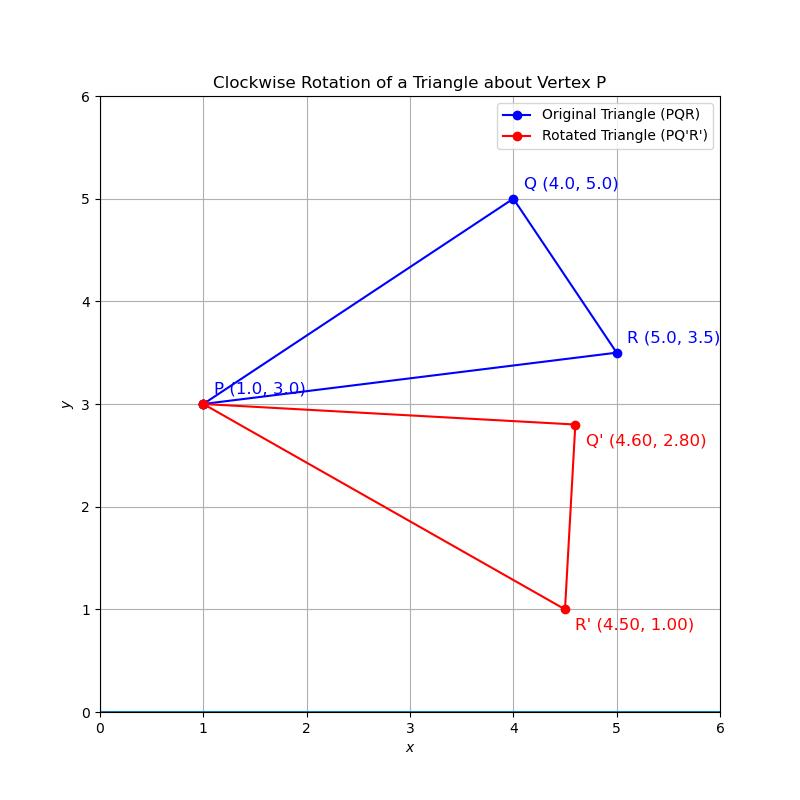
\includegraphics[width=0.5\columnwidth]{../figs/plot_c.jpg}
	\caption{Plot}
	\label{fig:fig}
\end{figure}
\end{frame}

\end{document}
